\chapter{Research Methodology and System Design}

This chapter outlines the research and engineering lifecycle, details stakeholder requirements, defines the functional and non-functional specifications, presents the multi-tiered system architecture, and formalizes the data flow diagrams and relational database entity-relationship schema.

\section{Research Methodology}
This project adopts an Agile Software Engineering lifecycle designed for iterative development, continuous validation, and rapid feedback integration. As illustrated in Figure~\ref{fig:methodology_pipeline}, the process comprises four iterative phases:

\begin{figure}[H]
\centering
\begin{tikzpicture}[
    node distance=1.6cm,
    block/.style={rectangle, draw=blue!70, fill=blue!10, text width=2.8cm, text centered, rounded corners, minimum height=1.2cm, font=\small\bfseries},
    arrow/.style={thick, ->, >=stealth}
]
\node[block] (req) {1. Requirements \& Domain Analysis};
\node[block, right=1.2cm of req] (arch) {2. System Architecture \& DB Modeling};
\node[block, right=1.2cm of arch] (impl) {3. Full-Stack Implementation};
\node[block, below=1.4cm of arch] (eval) {4. Empirical Testing \& Benchmarking};

\draw[arrow] (req) -- (arch);
\draw[arrow] (arch) -- (impl);
\draw[arrow] (impl) |- (eval);
\draw[arrow] (eval) -| (req);
\end{tikzpicture}
\caption{Iterative Agile Engineering and Validation Pipeline}
\label{fig:methodology_pipeline}
\end{figure}

\begin{enumerate}
    \item \textbf{Requirements Formulation}: Gathering operational constraints from university librarians, faculty members, and students to identify pain points in seat availability and book cataloging.
    \item \textbf{Architectural and Database Modeling}: Constructing relational schemas with composite unique constraints, defining RESTful API endpoints, and specifying data flow interactions.
    \item \textbf{Full-Stack Prototyping}: Implementing backend services using Express.js and TypeScript with Prisma ORM, coupled with a responsive Next.js 15 frontend.
    \item \textbf{Empirical Evaluation}: Conducting automated load testing, query latency benchmarks, and concurrency verification under high-volume stress conditions.
\end{enumerate}

\section{Stakeholder and Requirements Analysis}

\subsection{Stakeholder Analysis}
Table~\ref{tab:stakeholder_mapping} outlines the primary stakeholder groups interacting with the platform and their core operational expectations.

\begin{table}[H]
\centering
\caption{Stakeholder Analysis and System Needs Mapping}
\label{tab:stakeholder_mapping}
\small
\begin{tabularx}{\textwidth}{>{\raggedright\arraybackslash}p{2.8cm} >{\raggedright\arraybackslash}p{4.2cm} >{\raggedright\arraybackslash}X}
\toprule
\textbf{Stakeholder Group} & \textbf{Core Role / Context} & \textbf{System Needs \& Expectations} \\
\midrule
\textbf{Students} & Primary consumers of study spaces and academic literature & Real-time seat discovery, seamless slot booking, QR check-in, exact physical shelf location guidance, digital PDF reading/downloads, and online borrow renewals. \\
\textbf{Librarians / Staff} & Operational managers of physical desks and book circulation & Quick QR arrival verification, book issue and return processing, renewal request reviews, inventory status updates, and patron assistance. \\
\textbf{System Administrators} & Institutional system supervisors & Role-based user control, zone and seat grid setup, global lending policy configuration, audit logging, and aggregate utilization reports. \\
\bottomrule
\end{tabularx}
\end{table}

\subsection{Functional Requirements Specification (FRS)}
Table~\ref{tab:frs_matrix} specifies the core functional requirements governing system operations.

\begin{table}[H]
\centering
\caption{Functional Requirements Specification (FRS) Matrix}
\label{tab:frs_matrix}
\small
\begin{tabularx}{\textwidth}{>{\centering\arraybackslash}p{1.5cm} >{\raggedright\arraybackslash}p{3.8cm} >{\raggedright\arraybackslash}X >{\centering\arraybackslash}p{1.5cm}}
\toprule
\textbf{Req ID} & \textbf{Requirement Title} & \textbf{Functional Description} & \textbf{Priority} \\
\midrule
FR-01 & User Authentication & Role-based authentication (Admin, Librarian, Student) with JWT HttpOnly cookies and password hashing. & High \\
FR-02 & Seat Slot Reservation & Real-time interactive seat grid booking with concurrency protection against double-booking. & High \\
FR-03 & Dynamic QR Verification & Tokenized QR code check-in/check-out with automatic 15-minute no-show cancellation and email notification. & High \\
FR-04 & Physical Book Indexing & Multi-criteria search mapping books to exact coordinates (Floor, Block, Rack, Shelf position). & High \\
FR-05 & Digital PDF Repository & Uploading, previewing in-browser, and authorized downloading of electronic PDF versions of books. & High \\
FR-06 & Circulation Issuance & Staff-managed checkout workflow associating specific physical copy barcodes with student accounts. & High \\
FR-07 & Self-Service Renewal & Online student renewal requests validated against lending limits and approved/rejected by staff. & Medium \\
FR-08 & Zone \& Seat Management & Administrative creation, color-coding, rule definition, and maintenance toggling for zones and seats. & Medium \\
FR-09 & Slot Lifecycle Enforcer & 1-minute background cron worker issuing 10-min pre-expiration warnings and auto-releasing seats at slot end. & High \\
FR-10 & Admin Seat Cancellation & Administrative cancellation with mandatory/custom audit reasons and automated student alert emails. & High \\
FR-11 & Lending Policy Control & Global configuration of loan durations, max borrow limits, grace periods, and overdue penalties. & Medium \\
FR-12 & Reporting \& Analytics & Statistical analytics covering seat occupancy rates, popular books, and active circulation trends. & Low \\
\bottomrule
\end{tabularx}
\end{table}

\subsection{Non-Functional Requirements (NFR)}
\begin{itemize}
    \item \textbf{Performance}: API response latencies shall remain below 100\,ms for 95\% of requests under standard loads.
    \item \textbf{Data Integrity}: Strict ACID transactions preventing concurrent duplicate seat reservations ($0\%$ double-booking tolerance).
    \item \textbf{Security}: Passwords hashed using Bcrypt (salt rounds $\ge 10$), CSRF mitigation, and role-based route guards.
    \item \textbf{Usability \& Responsiveness}: Fully responsive interface optimized across mobile, tablet, and desktop viewports.
\end{itemize}

\section{System Architecture and Component Design}
The system implements a decoupled, modern three-tier web architecture as depicted in Figure~\ref{fig:system_architecture_diagram}.

\begin{figure}[H]
\centering
\begin{tikzpicture}[
    node distance=1.2cm and 1.5cm,
    tier/.style={rectangle, draw=gray!60, fill=gray!5, dashed, rounded corners, inner sep=12pt},
    box/.style={rectangle, draw=blue!80, fill=blue!10, text width=3.4cm, text centered, rounded corners, minimum height=1.1cm, font=\small\bfseries},
    dbbox/.style={cylinder, draw=green!70!black, fill=green!10, text width=3.0cm, text centered, shape border rotate=90, minimum height=1.3cm, font=\small\bfseries},
    conn/.style={thick, <->, >=stealth, color=blue!70!black}
]

% Presentation Layer
\node[box] (client1) {Student Portal\\(Next.js / Tailwind)};
\node[box, right=1.0cm of client1] (client2) {Staff \& Admin Desk\\(React 19 / Radix UI)};
\node[box, right=1.0cm of client2] (client3) {QR Scanner Module\\(Camera / Web APIs)};

% Business Logic Layer
\node[box, below=1.8cm of client1] (api_auth) {Auth \& RBAC Service\\(JWT / HttpOnly)};
\node[box, below=1.8cm of client2] (api_seat) {Seat \& Booking Engine\\(Slot Lock / QR Token)};
\node[box, below=1.8cm of client3] (api_book) {Book Index \& Circulation\\(Spatial Map / Loans)};

% Data Layer
\node[dbbox, below=1.8cm of api_seat] (postgres) {PostgreSQL DB\\(Prisma ORM Managed)};

% Connections
\draw[conn] (client1) -- (api_auth);
\draw[conn] (client1) -- (api_seat);
\draw[conn] (client1) -- (api_book);
\draw[conn] (client2) -- (api_seat);
\draw[conn] (client2) -- (api_book);
\draw[conn] (client3) -- (api_seat);

\draw[conn] (api_auth) -- (postgres);
\draw[conn] (api_seat) -- (postgres);
\draw[conn] (api_book) -- (postgres);

% Layer Labels
\node[above=0.2cm of client2, font=\large\bfseries, color=black!80] {Presentation Layer (Client-Side)};
\node[above=0.2cm of api_seat, font=\large\bfseries, color=black!80] {Application Layer (Express.js / TypeScript)};
\node[below=0.2cm of postgres, font=\large\bfseries, color=black!80] {Persistence Layer (PostgreSQL Database)};

\end{tikzpicture}
\caption{Three-Tier System Architecture Diagram}
\label{fig:system_architecture_diagram}
\end{figure}

\subsection{Core Subsystem Modules}
\begin{enumerate}
    \item \textbf{Seat Reservation Subsystem}: Manages zones, seat grids, slot schedules, real-time availability matrices, and automated status transitions (Confirmed $\rightarrow$ Checked-in $\rightarrow$ Completed / No-Show).
    \item \textbf{Automated Background Cron \& Notification Engine}: Multi-worker scheduling daemon operating on a 1-minute resolution to enforce 15-minute check-in grace periods, dispatch pre-expiration (10-minute) warning emails, execute slot-end seat release procedures, and notify students upon administrative cancellations.
    \item \textbf{Physical Book Indexing Engine}: Resolves book searches to concrete bookshelf coordinates ($\text{Floor} \rightarrow \text{Block} \rightarrow \text{Rack} \rightarrow \text{Shelf Position}$), displaying spatial navigation cues.
    \item \textbf{Digital Media \& Book Catalog Subsystem}: Houses bibliographic records with cloud-hosted high-resolution cover images managed via Cloudinary CDN and in-memory Multer streams, incorporating automated asset deletion rollbacks on failed transactions, alongside digital PDF document reading and downloads.
    \item \textbf{Circulation \& Renewal Engine}: Manages lending transactions, due dates, renewal request validation, and overdue tracking with complete administrative governance.
\end{enumerate}

\section{Hardware Bill of Materials (BOM) and Deployment Cost}
Table~\ref{tab:hardware_bom} details the deployment and operational infrastructure budget for campus-wide rollout.

\begin{table}[H]
\centering
\caption{Infrastructure and Hardware Bill of Materials (BOM)}
\label{tab:hardware_bom}
\small
\begin{tabularx}{\textwidth}{>{\raggedright\arraybackslash}p{3.2cm} >{\raggedright\arraybackslash}X >{\raggedright\arraybackslash}X >{\raggedleft\arraybackslash}p{2.2cm}}
\toprule
\textbf{Component / Service} & \textbf{Model / Specifications} & \textbf{Operational Role} & \textbf{Est. Cost (BDT)} \\
\midrule
Cloud Application VPS & 4 vCPU, 8GB RAM, SSD Storage (Ubuntu) & Hosting Express backend and Next.js frontend & 18,000 / yr \\
Managed PostgreSQL & Scalable Managed PostgreSQL 16 & Relational database storage with daily snapshots & 12,000 / yr \\
Circulation QR Scanners & 2D Optical Barcode / QR Scanner Units & Staff desk check-in and checkout processing & 8,500 \\
Library Entry Tablets & 10-inch Android Wall-Mount Tablets & Student self-service seat check-in kiosk & 24,000 \\
Domain \& SSL Security & Enterprise TLS 1.3 / Custom Domain & Encrypted HTTPS transmission & 3,500 / yr \\
\midrule
\multicolumn{3}{l}{\textbf{Total Initial Deployment Cost}} & \textbf{66,000 BDT} \\
\bottomrule
\end{tabularx}
\end{table}

\section{Data Flow Modeling (DFD)}

\subsection{Context Diagram (DFD Level 0)}
Figure~\ref{fig:dfd_level_0} depicts the Level 0 Context Diagram showing external entities (Students, Staff/Librarians, Administrators) interacting with the boundary of the Smart Library Management System.

\begin{figure}[H]
\centering
\begin{tikzpicture}[
    node distance=2.2cm and 2.5cm,
    entity/.style={rectangle, draw=blue!80, fill=blue!10, text width=2.4cm, text centered, minimum height=1.0cm, font=\small\bfseries},
    process/.style={circle, draw=green!70!black, fill=green!10, text width=3.2cm, text centered, minimum size=3.2cm, font=\small\bfseries},
    flow/.style={thick, ->, >=stealth, font=\footnotesize}
]
\node[process] (sys) {0.0\\Smart Library\\Management\\System};
\node[entity, left=of sys] (stu) {Student};
\node[entity, above=of sys] (adm) {Administrator};
\node[entity, right=of sys] (lib) {Librarian / Staff};

\draw[flow] (stu) -- node[above, text width=2.2cm, text centered] {Seat booking, Search book, Renew request} (sys);
\draw[flow] (sys) -- node[below, text width=2.2cm, text centered] {QR Pass, Shelf location, PDF file} (stu);

\draw[flow] (adm) -- node[left, text width=2.2cm, text centered] {Configure zones, User roles, Settings} (sys);
\draw[flow] (sys) -- node[right, text width=2.2cm, text centered] {Audit logs, Analytics} (adm);

\draw[flow] (lib) -- node[above, text width=2.2cm, text centered] {Issue books, Return, Verify QR} (sys);
\draw[flow] (sys) -- node[below, text width=2.2cm, text centered] {Circulation status, Overdue alerts} (lib);

\end{tikzpicture}
\caption{Level 0 Context Data Flow Diagram}
\label{fig:dfd_level_0}
\end{figure}

\subsection{Decomposed Data Flow Diagram (DFD Level 1)}
The decomposed Level 1 DFD segregates system operations into discrete functional processes:
\begin{itemize}
    \item \textbf{Process 1.0 (Authentication \& Role Verification)}: Validates student and staff credentials, issuing encrypted JWT tokens.
    \item \textbf{Process 2.0 (Seat Scheduling \& Concurrency Lock)}: Checks schedule slot availability, applies unique constraints, and issues tokenized QR passes.
    \item \textbf{Process 3.0 (QR Arrival Verification \& Attendance)}: Decrypts QR tokens, matches timestamps against active windows, and transitions booking states.
    \item \textbf{Process 4.0 (Bibliographic Search \& Shelf Coordinate Resolution)}: Queries book records and retrieves multi-tier physical coordinates (Floor, Block, Rack, Shelf).
    \item \textbf{Process 5.0 (Circulation \& Renewal Pipeline)}: Processes checkout loans, tracks due dates, and manages renewal requests.
    \item \textbf{Process 6.0 (Automated Notification \& Seat Reclamation Engine)}: Evaluates active time windows, dispatches transactional emails for cancellations and expiration warnings, and auto-releases physical seats.
\end{itemize}

\section{Database Design and Relational Schema (ERD)}
The database architecture is designed with high normalization (3NF) to eliminate data redundancy while enforcing relational referential integrity. Figure~\ref{fig:relational_erd} illustrates the Entity-Relationship Diagram.

\begin{figure}[H]
\centering
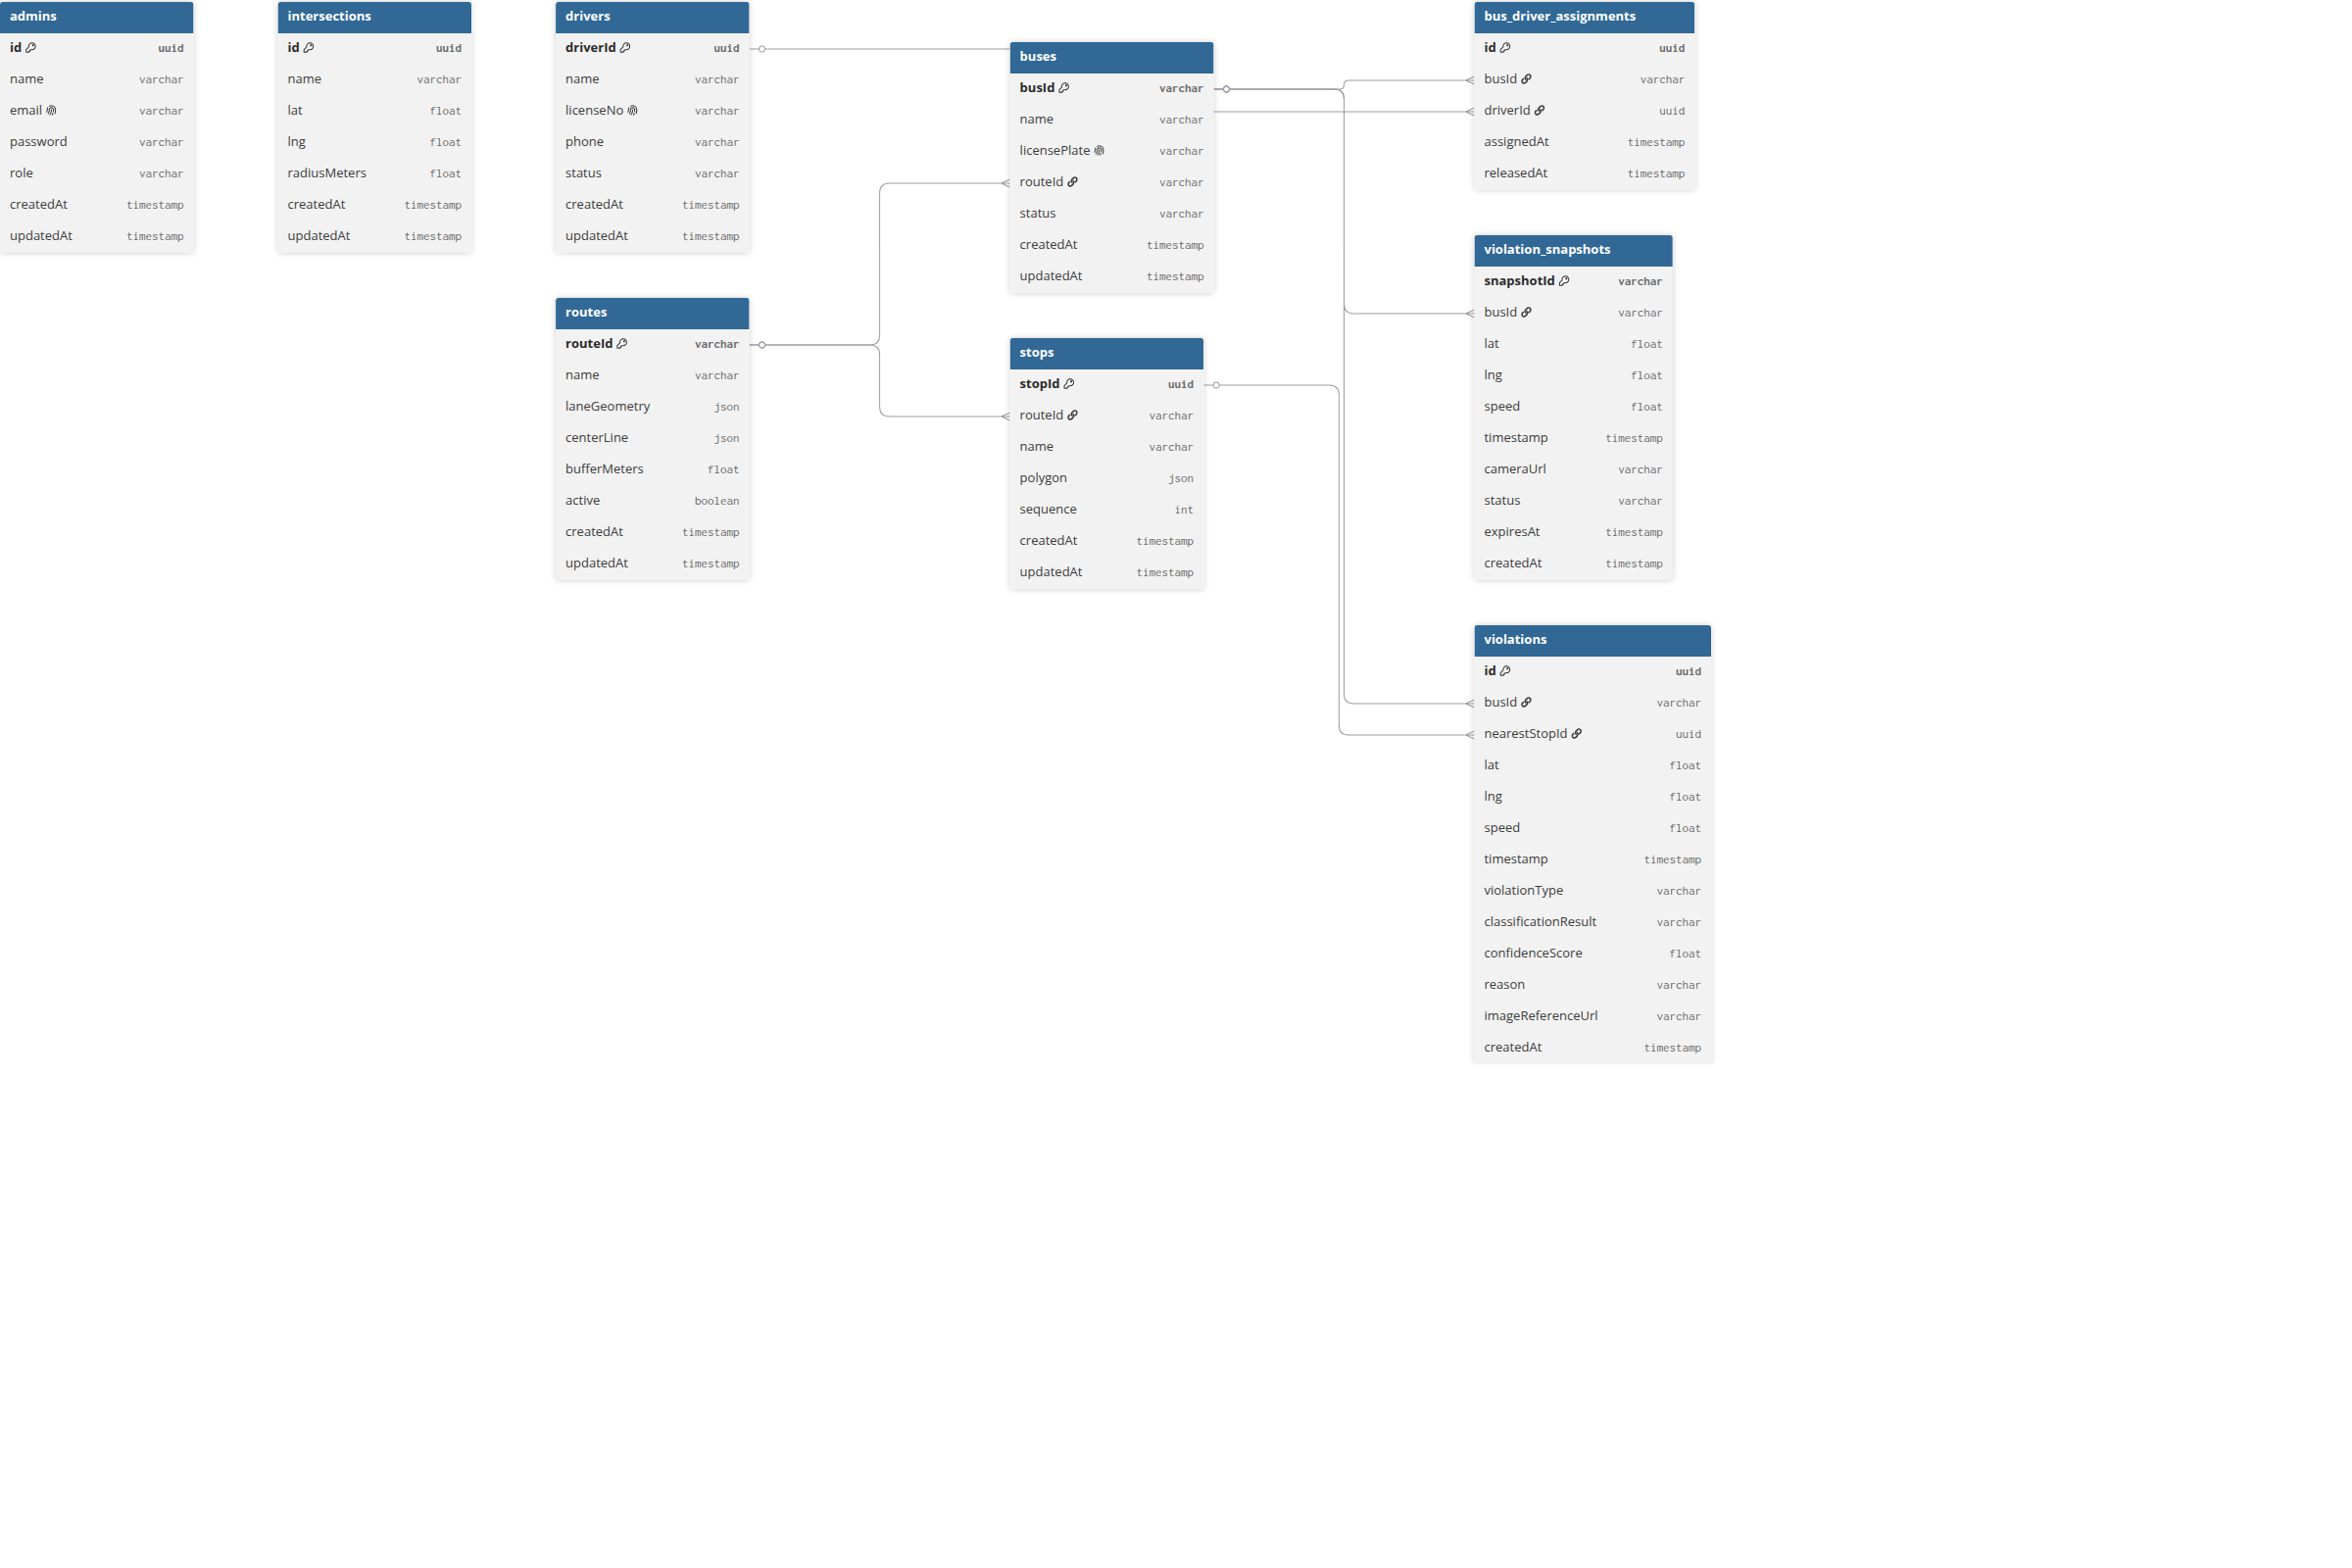
\includegraphics[width=0.95\textwidth]{./media/final_ERD.png}
\caption{Complete Relational Entity-Relationship Diagram (ERD)}
\label{fig:relational_erd}
\end{figure}

\subsection{Relational Entity Specifications}
\begin{itemize}
    \item \textbf{User}: Stores identity attributes, hashed credentials, and role enumerations (\texttt{admin}, \texttt{librarian}, \texttt{student}).
    \item \textbf{Zone \& Seat}: Defines physical study zones with color tags, rules, and individual seats uniquely constrained by \texttt{[zoneId, seatNumber]}.
    \item \textbf{Schedule \& Booking}: Manages discrete daily time slots (\texttt{morning}, \texttt{noon}, \texttt{afternoon}, \texttt{evening}) and seat reservations with composite unique key \texttt{[seatId, scheduleId]} to prevent double-booking. Tracks reservation lifecycles via \texttt{status}, \texttt{qrToken}, \texttt{bookedAt}, \texttt{checkedInAt}, \texttt{checkedOutAt}, \texttt{cancelledAt}, \texttt{cancelReason}, and \texttt{slotWarningEmailSent}.
    \item \textbf{Book \& Category}: Houses bibliographic metadata (ISBN, title, author, edition, description, cover image URL, PDF URL) linked to specific thematic categories.
    \item \textbf{ShelfLocation \& BookCopy}: Maps individual physical copies (identified by unique barcodes) to spatial coordinates: \texttt{floor}, \texttt{blockNumber}, \texttt{rackNumber}, and \texttt{shelfPosition}.
    \item \textbf{BookLoan}: Tracks lending lifecycles, due dates, return timestamps, renewal counters, overdue fine statuses, payment methods, and automated email reminder tracking flags (\texttt{warningEmailSent}, \texttt{overdueEmailSent}).
\end{itemize}
